\begin{tikzpicture}
\node[anchor=south west,inner sep=0] at (0,0) {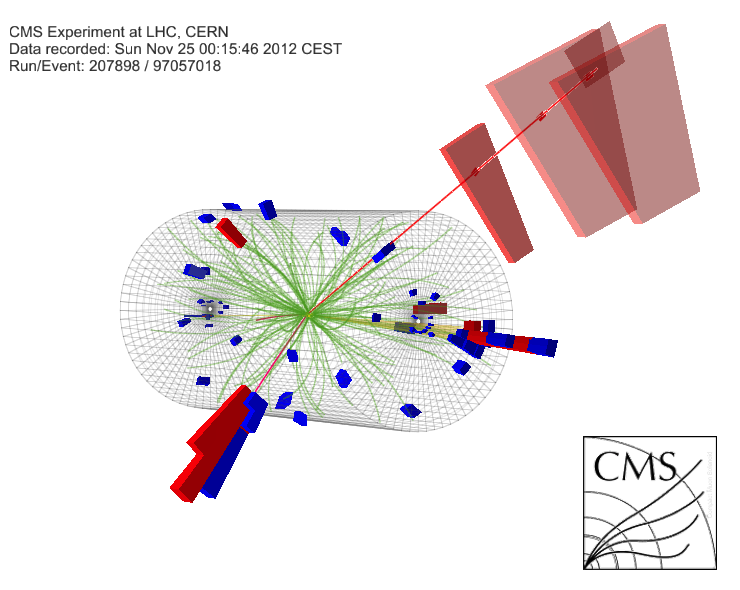
\includegraphics[width=10cm, trim = 0cm 7mm 0cm 7mm, clip]{\PhDthesisdir/plots_and_images/Event_displays/run207898_white_3d_filtered.png}};

\draw (10.5, 7) node (L1) {\LARGE\mu} ;
\draw [thick, -latex] (L1) --+(-170:1);

\draw (1.5, 0) node (L2) {\LARGE\tauh} ;
\draw [thick, -latex] (L2) --+(45:1);

\draw [red] (0, 1.25) node [right] (ECAL) {ECAL deposit} ;
\draw [thick, -latex, red] (ECAL) -- (2.5,1.5);

\draw [blue] (3.5, .5) node [right] (HCAL) {HCAL deposit} ;
\draw [thick, -latex, blue] (HCAL) -- (3.125,1.25);

\draw [ltcolorgreen] (0, 4) node [right] (trk) {tracks} ;
\draw [thick, -latex, ltcolorgreen4] (trk) -- (3.5,2.75);
\draw [thick, -latex, ltcolorgreen4] (trk) -- (4.75,4);

\draw [ltcolorred] (9, 3.5) node (mu) {muon chambers} ;
\draw [thick, -latex, ltcolorred] (mu) -- (8.5,4.5);

\draw [ltcolorgray] (2.5, 6) node (trkvol) {tracker volume} ;
\draw [thick, -latex, ltcolorgray] (trkvol) -- (4, 5);
\end{tikzpicture}